\documentclass{llncs}

\usepackage{graphicx,epsfig,amssymb,amsmath,todonotes}
\usepackage{mathpartir}
\usepackage{xspace}
%\usepackage[colorlinks=true]{hyperref}
\usepackage[colorlinks=true,linkcolor=black,citecolor=black,urlcolor=black]{hyperref}
\usepackage{algorithm,algpseudocode}
\usepackage{tikz}
\usepackage{subcaption}

\usepackage[utf8]{inputenc}
\usepackage{newunicodechar}
\newunicodechar{∃}{\ensuremath{\exists}}
\newunicodechar{∀}{\ensuremath{\forall}}
\newunicodechar{θ}{\ensuremath{\theta}}
\newunicodechar{τ}{\ensuremath{\tau}}
\newunicodechar{φ}{\ensuremath{\varphi}}
\newunicodechar{π}{\ensuremath{\pi}}
\newunicodechar{α}{\ensuremath{\alpha}}
\newunicodechar{β}{\ensuremath{\beta}}
\newunicodechar{γ}{\ensuremath{\gamma}}
\newunicodechar{δ}{\ensuremath{\delta}}
\newunicodechar{ε}{\ensuremath{\epsilon}}
\newunicodechar{λ}{\ensuremath{\lambda}}
\newunicodechar{ρ}{\ensuremath{\rho}}
\newunicodechar{σ}{\ensuremath{\sigma}}
\newunicodechar{ω}{\ensuremath{\omega}}
\newunicodechar{Γ}{\ensuremath{\Gamma}}
\newunicodechar{Φ}{\ensuremath{\Phi}}
\newunicodechar{Δ}{\ensuremath{\Delta}}
\newunicodechar{Σ}{\ensuremath{\Sigma}}
\newunicodechar{Π}{\ensuremath{\Pi}}
\newunicodechar{Θ}{\ensuremath{\Theta}}
\newunicodechar{⇒}{\ensuremath{\Rightarrow}}
\newunicodechar{⇐}{\ensuremath{\Leftarrow}}
\newunicodechar{⇔}{\ensuremath{\Leftrightarrow}}
\newunicodechar{→}{\ensuremath{\rightarrow}}
\newunicodechar{←}{\ensuremath{\leftarrow}}
\newunicodechar{↔}{\ensuremath{\leftrightarrow}}
\newunicodechar{¬}{\ensuremath{\neg}}
\newunicodechar{∧}{\ensuremath{\land}}
\newunicodechar{∨}{\ensuremath{\lor}}
\newunicodechar{≠}{\ensuremath{\neq}}
\newunicodechar{≡}{\ensuremath{\equiv}}
\newunicodechar{∼}{\ensuremath{\sim}}
\newunicodechar{≈}{\ensuremath{\approx}}
\newunicodechar{≥}{\ensuremath{\geq}}
\newunicodechar{≤}{\ensuremath{\leq}}
\newunicodechar{≫}{\ensuremath{\gg}}
\newunicodechar{≪}{\ensuremath{\ll}}
\newunicodechar{∅}{\ensuremath{\emptyset}}
\newunicodechar{⊆}{\ensuremath{\subseteq}}
\newunicodechar{⊂}{\ensuremath{\subset}}
\newunicodechar{∩}{\ensuremath{\cap}}
\newunicodechar{∪}{\ensuremath{\cup}}
\newunicodechar{∈}{\ensuremath{\in}}
\newunicodechar{⊤}{\ensuremath{\top}}
\newunicodechar{⊥}{\ensuremath{\bot}}
\newunicodechar{₀}{\ensuremath{_0}}
\newunicodechar{₁}{\ensuremath{_1}}
\newunicodechar{₂}{\ensuremath{_2}}
\newunicodechar{₃}{\ensuremath{_3}}
\newunicodechar{₄}{\ensuremath{_4}}
\newunicodechar{₅}{\ensuremath{_5}}
\newunicodechar{₆}{\ensuremath{_6}}
\newunicodechar{₇}{\ensuremath{_7}}
\newunicodechar{₈}{\ensuremath{_8}}
\newunicodechar{₉}{\ensuremath{_9}}
\newunicodechar{⁰}{\ensuremath{^0}}
\newunicodechar{¹}{\ensuremath{^1}}
\newunicodechar{²}{\ensuremath{^2}}
\newunicodechar{³}{\ensuremath{^3}}
\newunicodechar{⁴}{\ensuremath{^4}}
\newunicodechar{⁵}{\ensuremath{^5}}
\newunicodechar{⁶}{\ensuremath{^6}}
\newunicodechar{⁷}{\ensuremath{^7}}
\newunicodechar{⁸}{\ensuremath{^8}}
\newunicodechar{⁹}{\ensuremath{^9}}
\newunicodechar{𝔹}{\ensuremath{\mathbb{B}}}
\newunicodechar{ℝ}{\ensuremath{\mathbb{R}}}
\newunicodechar{ℕ}{\ensuremath{\mathbb{N}}}
\newunicodechar{ℂ}{\ensuremath{\mathbb{C}}}
\newunicodechar{ℚ}{\ensuremath{\mathbb{Q}}}
\newunicodechar{ℤ}{\ensuremath{\mathbb{Z}}}
\newunicodechar{✓}{\checkmark}
\newunicodechar{✗}{\ensuremath{\times}}
\newunicodechar{◊}{\ensuremath{\lozenge}}
\newunicodechar{□}{\ensuremath{\square}}

\newcommand{\thLemI}{\textsf{ThLem-I}\xspace}
\newcommand{\thLem}{\textsf{ThLem}\xspace}
\newcommand{\spltI}{\textsf{Split-I}\xspace}
\newcommand{\splt}{\textsf{Split}\xspace}
\newcommand{\weaken}{\textsf{Weakening}\xspace}
\newcommand{\weakenI}{\textsf{Weakening-I}\xspace}

\newcommand{\entails}{~\ensuremath{\vdash}~}

\newcommand{\dReal}{\textsf{dReal}\xspace}%dreal3 will become dreal during the reviewing time :)
\newcommand{\zthree}{\textsf{Z3}\xspace}
\newcommand{\mathsat}{\textsf{MathSat5}\xspace}
\newcommand{\smtinterpol}{\textsf{SmtInterpol}\xspace}
\newcommand{\princess}{\textsf{Princess}\xspace}
\newcommand{\iSat}{\textsf{iSat}\xspace}


\newcommand{\lrf}{\mathcal{L}_{\mathbb{R}_{\mathcal{F}}}}
%\newtheorem{definition}{Definition}
\newtheorem{notation}{Notation}
%\newtheorem{example}{Example}
%\newtheorem{proposition}{Proposition}
%\newtheorem{remark}{Remark}
%\newtheorem{theorem}{Theorem}

\begin{document}

% we have 15 pages + 2 pages biblio

\title{Interpolants in Nonlinear Theories over the Reals}
\author{Sicun Gao \and Damien Zufferey\thanks{Sicun Gao was supported by NSF (Grant CCF-1161775 and CPS-1446725). 
Damien Zufferey was supported by NSF (Grant CCF-1138967) and DARPA (Grant FA8650-15-C-7564).}}

\institute{MIT}

\maketitle

\begin{abstract}
We develop an algorithm for computing Craig interpolants for first-order formulas over real numbers with a wide range of nonlinear functions, including transcendental functions and differential equations.
We transform proof traces from δ-complete decision procedures into interpolants that consist of Boolean combinations of linear constraints.
The algorithms are guaranteed to find the interpolants between two formulas $A$ and $B$ whenever $A ∧ B$ is not δ-satisfiable.
At the same time, by exploiting δ-perturbations one can parameterize the algorithm to find interpolants with different positions between $A$ and $B$.
We show applications of the methods in geometric theorem proving, robotic design, and hybrid system verification.  

\end{abstract}

\section{Introduction}
\label{sec:intro}

%Software often interact with the physical world. Plant controllers, robots, cars, etc., all theses systems contains sensors and actuators. Validating such systems requires requires method to reason not only about the software part, but also the environment, usually described by continuous equations.

Verification problems of complex embedded software can be reduced to solving logic formulas that contain continuous, typically nonlinear, real functions. The framework of δ-decision procedures~\cite{DBLP:conf/lics/GaoAC12,DBLP:conf/fmcad/GaoKC13} establishes that, under reasonable relaxations, nonlinear SMT formulas over the reals are in principle as solvable as SAT problems. Indeed, using solvers for nonlinear theories as the algorithmic engines, straightforward bounded model checking has already shown promise on nonlinear hybrid systems~\cite{DBLP:conf/cav/ChenAS13,DBLP:conf/tacas/KongGCC15}. Naturally, for enhancing performance, more advanced reasoning techniques need to be introduced, extending SMT towards general quantifier elimination. However, it is well-known that quantifier elimination is not feasible for nonlinear theories over the reals\footnote{Quantifier elimination for real arithmetic (i.e., with polynomials only) is computable but the complexity is too high for most practical applications. If transcendental functions are involved, the problem is highly undecidable.}.  

Craig interpolation is a weak form of quantifier elimination.
Given two formulas $A$ and $B$, such that $A ∧ B$ is unsatisfiable, an interpolant $I$ is a formula satisfying: (1) $A ⇒ I$, (2) $B ∧ I ⇒ ⊥$, and (3) $I$ contains only variables common to $A$ and $B$.
It has found many applications in verifications:
as an heuristic to compute inductive invariant~\cite{DBLP:conf/cav/McMillan03,DBLP:conf/vmcai/McMillan07,DBLP:conf/sas/McMillan11},
for predicate discovery in abstraction refinement loops~\cite{DBLP:conf/cav/McMillan06},
inter procedural analysis~\cite{DBLP:conf/vmcai/AlbarghouthiGC12,DBLP:conf/cav/AlbarghouthiLGC12},
shape analysis~\cite{DBLP:conf/esop/AlbarghouthiBCK15},
fault-localisation~\cite{DBLP:conf/fm/ErmisSW12,DBLP:conf/vmcai/ChristESW13,DBLP:conf/sigsoft/SchafSW13}, and so on.

In this paper, we present methods for computing Craig interpolants in expressive nonlinear theories over the reals. To do so, we extract interpolants from proofs of unsatisfiability generated by δ-decision procedures~\cite{DBLP:conf/synasc/GaoKC14} based on Interval Constraint Propagation (ICP)~\cite{handbookICP}. The proposed algorithms are guaranteed to find the interpolants between two formulas $A$ and $B$ whenever $A ∧ B$ is not δ-satisfiable.

δ-decision problems relax the standard notion of logical decisions by allowing one-sided δ-bounded errors~\cite{DBLP:conf/lics/GaoAC12,DBLP:conf/cade/GaoAC12}. Instead of asking whether a formula has a satisfiable assignment or not, we ask if it is ``{\em δ-satisfiable}" or ``unsatisfiable". Here, a formula is δ-satisfiable if it would be satisfiable under some {\em δ-perturbation} on the original formula~\cite{DBLP:conf/cade/GaoAC12}. On the other hand, when the algorithm determines that the formula is ``unsatisfiable", no numerical error can be involved. Indeed, we can extract proofs of unsatisfiability from such answers, even though the search algorithms involve numerical errors~\cite{DBLP:conf/synasc/GaoKC14}. This is accomplished by analyzing the execution trace of the search tree based on the ICP algorithm. 


The core ICP algorithm uses a {\em branch-and-prune} loop that aims to either find a small enough box that witnesses δ-satisfiability, or detect that no δ-solutions exists. The loop consists of two main steps:
\begin{itemize}
\item (Prune) Use interval arithmetic to maintain overapproximations of the solution sets, so that one can ``prune" out the part of the state space that does not contain solutions.
\item (Branch) When the pruning operation does not make progress, one performs a depth-first search by ``branching" on variables and restart pruning operations on a subset of the domain. 
\end{itemize}
The loop is continued until either a small enough box that may contain a solution is found, or any conflict among the constraints is observed.

\begin{figure}
\centering
\includegraphics[scale=0.04]{img/example.pdf}
\caption{
    Interval constraint propagation and interpolant construction where $A$ is $y≥x²$ and $B$ is $y ≤ -\cos(x) + 0.8$ over the domain $x∈[-1,1]$, $y∈[-1,1]$.
    The $A$ is shown in green and $B$ in red.
    The final interpolant is the green part.
}
\label{fig:example}
\end{figure}


When a formula is unsatisfiable, the execution trace of the algorithm becomes can be seen as a proof tree that divides the space into small hypercubes and associating a constraint to each hypercube~\cite{DBLP:conf/synasc/GaoKC14}. Consequently, the interpolation algorithm can traverse this proof tree to construct the interpolant. To each leaf in the proof, we associate ⊤ or ⊥ depending on the source of the contradiction. The inner nodes of the proof tree correspond to case splits and are handled in a manner reminiscent of Pudl{\'a}k's algorithm~\cite{MR1472134}. Common variables are kept as branching points and $A$,$B$ local variables are eliminated. A simple example of the method is as follows:

\begin{example}
Let $A$ be $y≥x²$ and $B$ by $y ≤ -\cos(x) + 0.8$ over the domain $x∈[-1,1]$, $y∈[-1,1]$.
A δ-decision procedure uses $A$ and $B$ to contract the domains of $x$ and $y$ by removing the parts that be shown empty using interval arithmetic.
Figure~\ref{fig:example} shows a sequence of contraction proving the unsatisfiability of the formula.
As the contraction occurs, we color the region of the space by the color of the \emph{opposite} formula.
When the interval constraint propagation has finished the initial domain is associated to either $A$ or $B$.
The interpolant $I$ is composed of the parts corresponding to $A$.
$I$ is $y ≥ 0 ∧ (0.26 ≤ y ∨ (y ≤ 0.26 ∧ -0.51 ≤ x ≤ 0.51))$.
\end{example}

We have implemented the algorithms in the SMT solver \dReal~\cite{DBLP:conf/cade/GaoKC13}. We show examples of applications from various domains such as control and robotic design, and hybrid system verification.  

\paragraph{Related work.}
Our algorithm is surprisingly similar to the algorithm for propositional interpolation studied by Pudl{\'a}k~\cite{MR1472134}.
However, it applies to a different theory.
Craig interpolation for real or integer arithmetic has focused on the linear fragment with LA(ℝ)~\cite{DBLP:conf/tacas/McMillan04,DBLP:conf/vmcai/RybalchenkoS07} and LA(ℤ)~\cite{DBLP:conf/cade/BrilloutKRW10,DBLP:conf/tacas/GriggioLS11}.
Our method currently handles nonlinear fragments over ℝ.

Existing tools to compute interpolation such as
\mathsat~\cite{mathsat5},
\princess~\cite{DBLP:conf/cade/BrilloutKRW10},
\smtinterpol~\cite{DBLP:conf/spin/ChristHN12}, and
\zthree~\cite{DBLP:conf/fmcad/McMillan11}
focus on linear arithmetic.
We are the first to provide interpolation in nonlinear theories.


\paragraph{Outline.}
In Section~\ref{sec:prelim}, we review notions related to interpolation, nonlinear arithmetic over the Reals and δ-decision procedures.
In Section~\ref{sec:itp}, we introduce our interpolation algorithm.
In Section~\ref{sec:eval}, we present and evaluate our implementation.
Finally, we conclude and sketch future research direction in Section~\ref{sec:concl}.

%Given two formulas which conjunction is unsatisfiable, the Craig interpolant~\cite{MR0104564} is a formula over the common variables that serves

%reasoning about the combined system of software and the physical environment. Modeling such environment typically requires extensive use of continuous functions over real numbers, such as solution functions of nonlinear differential equations. Thus solving logic formulas in nonlinear theories over the real numbers is a basic requirement for verification. 
%Unfortunately, automated reasoning for about nonlinear systems of equations is a hard, even undecidable in the general case~\cite{DBLP:conf/lics/GaoAC12}.
%However, recently the point of view~\cite{realQuasiDec,hybridQuasiDec} where reals are considered up to a certain precision was used to show decidability of the satisfiability for non-linear real arithmetic
%The intuition is that well engineered systems are robust, thus, are able to deal with small perturbations.

%In the δ-satisfiability framework, a system of equations is unsatisfiable if it does not have solution even when perturbed up to a δ constant. The complexity of δ-satisfiability is NP without ODE~\cite{DBLP:conf/lics/GaoAC12} and PSpace with ODE~\cite{DBLP:conf/fmcad/GaoKC13}. Furthermore, δ-satisfiability can leverage on the finite precision arithmetic for efficient implementations.

\section{Preliminaries}
\label{sec:prelim}

\paragraph{Craig interpolation~\cite{MR0104564}.}
We consider Craig interplants for quantifier-free first-order formulas. Given two formulas $A$ and $B$, such that $A ∧ B$ is unsatisfiable, an interpolant $I$ is a formula satisfying:
\begin{itemize}
\item $A ⇒ I$;
\item $B ∧ I ⇒ ⊥$;
\item $fv(I) ⊆ fv(A) ∩ fv(B)$ where $fv(\cdot)$ returns the free variables in a formula.
\end{itemize}
\begin{notation}
We use the meta-level symbol $\Rightarrow$ as a shorthand for logical implications in texts. In the proof rules that we will introduce shortly, $\vdash$ is used as the formal symbol with the standard interpretation as logical derivations. 
\end{notation}

\paragraph{Delta-Complete Decision Procedures.}

We consider first-order formulas interpreted over the real numbers. Our special focus is formulas that can contain arbitrary nonlinear functions that are {\em Type 2 computable}~\cite{CAbook,vasco}. Intuitively, Type 2 computability corresponds to {\em numerical computability}. For our purpose, it is enough to note that this set of functions consist of all common elementary functions, as well as solutions of Lipschitz-continuous ordinary differential equations. 

Interval Constraint Propagation (ICP)~\cite{handbookICP} finds
solutions of real constraints using the \emph{branch-and-prune} method, combining
interval arithmetic and constraint propagation. The idea is to use interval
extensions of functions to \emph{prune} out sets of points that are not in the
solution set and \emph{branch} on intervals when
such pruning can not be done, recursively until a small enough box
that may contain a solution is found or inconsistency is observed.
A high-level description of the decision version of ICP is given in Algorithm~\ref{icpalgo}~\cite{handbookICP,DBLP:conf/cade/GaoAC12}.
The boxes, or interval domains, are written as $\vec D$ and $c_i$ denotes the $i$th constraint.
\begin{algorithm}\label{algo1}
\caption{ICP($c_1,...,c_m, \vec D = D_1\times\cdots\times D_n, \delta$)}\label{icpalgo}
\begin{algorithmic}[1]
\Statex
    \State $S \gets \vec D$
    \While{$S \neq \emptyset$}
        \State $\vec D \gets S.\mathrm{pop}()$
        \While{$\exists 1 \leq i \leq m, \vec D \neq_{\delta} \mathrm{Prune}(\vec D,c_i)$}
        \State $\vec D \gets \mathrm{Prune}(\vec D, c_i)$
        \EndWhile
        \If{$\vec D \neq \emptyset$}
            \If{$\exists 1\leq i\leq m, |\vec D|\geq \varepsilon$} \Comment{$\varepsilon$ is some computable factor of $\delta$}
                \State $\{\vec D_1,\vec D_2\} \gets \mathrm{Branch}(\vec D, i)$
                \State $S.\mathrm{push}(\vec D_1)$
                \State $S.\mathrm{push}(\vec D_2)$
            \Else
                \State \Return {\sf sat}
            \EndIf
        \EndIf
    \EndWhile
    \State \Return {\sf unsat}
\end{algorithmic}
\end{algorithm}

\begin{example}
Consider a constraint $c(x,y) : y=x \wedge y = x^2$, and $x\in [1.5,2]$ and
$y\in [1,2]$ are the initial interval assignment. We use the abstract-DPLL style notation $\vec x\in \vec D||c$ to denote the pair of the sequence of interval assignments. (For more details, see~\cite{DBLP:conf/synasc/GaoKC13}.) A run of the ICP algorithm on this problem is as follows:
\begin{eqnarray*}
& &x\in [1.5,2], y\in [1,2]\parallel c \\
&\stackrel{branch}{\Longrightarrow}& x\in [1.5,2],
y\in [1,2], (x\in [1.7, 2])^d\parallel c\\
& &\mbox{  (branching on the x variable, looking only at the part $x\in[1.7,2]$)}\\
&\stackrel{backtrack}{\Longrightarrow}& x\in [1.5,2], y\in [1,2], x\in [1.5, 1.7]\parallel c\\
& &\mbox{  (backtracking, since $\forall\vec a\in [1.7,2]\times [1,2]$,
$c(\vec a)$ is false,}\\
& & \hspace{4cm} \mbox{and $[1.5,2]\subseteq[1.5,1.7]\cup [1.5, 2]$ for
$x$)}\\
&\stackrel{prune}{\Longrightarrow}& x\in [1.5,2], y\in [1,2], x\in [1.5, 1.7], x\in
[1.5, 1.6]\parallel c\\
& & \mbox{  (pruning, since $\forall \vec a\in[1.6,1.7]\times [1, 2]$, $c(\vec
a)$ is false)}\\
&\stackrel{prune}{\Longrightarrow}& x\in [1.5,2], y\in [1,2], x\in [1.5, 1.7],x\in [1.5, 1.6], x\in \emptyset\parallel c\\
& & \mbox{  (pruning, since $\forall \vec a\in[1.5,1.6]\times [1, 2]$, $c(\vec
a)$
is false)}\\
&\stackrel{fail}{\Longrightarrow}& \emptyset||c\ \mbox{ (since
$\forall \vec a\in \emptyset \times [1, 2], c(\vec a)$ is false.)}
\end{eqnarray*}
In the last step, the algorithm concludes that there is a conflict between the assignment sequence and the constraint, because $x\in \emptyset$ has been derived. 
\end{example}

\paragraph{Proofs from constraint propagation.}

The complete theory behind proof extraction from $\delta$-decision procedure is available in~\cite{DBLP:conf/synasc/GaoKC14}.
Here, we described a simplified version.
The proof is divides the solution space until it can prove, using interval arithmetic, that each small piece of the solution space is empty.
The solver uses constraints propagation and pruning steps to limit the amount of branching required.
However, the proof it produces only need to consider two main rules: splitting and theory lemma.
The rules are shown in Figure~\ref{fig:rules}.
The \splt rules divides the solution space into two disjoint subspaces.
The theory lemmas (\thLem) are the leaves of the proof.
They occurs when the solver managed to prove the absence of solution in a given subspace.
The interval constraints propagation algorithms works on one constraint at the time. 
The \weaken rule extracts those conjunct out of the main formula.

Each step of the proof has a set of variables $\vec x$ with a domain $\vec D$ and $F$ is a formula.
We use of vectors in the formulas, writing $\vec x ∈ \vec D$ to denote $\bigwedge_i x_i ∈ D_i$.
The domains are intervals, i.e., each $D_i$ has the form $[l_i,u_i]$ where $l_i$,$u_i$ are the lower and upper bounds for $x_i$.
Since we are looking at unsatisfiability proofs, each node implies $⊥$.

The root of the proof is has formula $A ∧ B$ and $D$ covers the entire domain,
the inner nodes are \splt.
and the proof's leaves are theory lemmas directly followed by a weakening.

\begin{notation}
In the proof rules, we use the standard notations for sequent calulus. Also, when we write an interval $[a,b]$, we always assume that it is a well-defined real interval satisfying $a\leq b$. 
\end{notation}

\begin{figure}
\centering
\begin{mathpar}
\inferrule{ {} }{
  \vec x ∈ \vec D ∧ c \entails ⊥
}{(\thLem)}\\

\inferrule{
  C := c ∧ \bigwedge_k C_k \\
  \vec x ∈ \vec D ∧ c \entails ⊥
}{
  \vec x ∈ \vec D ∧ C \entails ⊥
}{(\weaken)}\\

\inferrule{
  x_i ∈ [l_i, p] ∧ \bigwedge_{j ≠ i} x_j ∈ D_j ∧ C \entails ⊥ \\
  x_i ∈ [p, u_i] ∧ \bigwedge_{j ≠ i} x_j ∈ D_j ∧ C \entails ⊥
}{
  x_i\in [l_i, u_i] \wedge \bigwedge_{j\neq i} x_j∈ D_j ∧ C \entails ⊥
}{(\splt)}
\end{mathpar}
\caption{Proof rules for the ICP algorithm}
\label{fig:rules}
\end{figure}

Algorithm~\ref{icpalgo} generates proof during the \emph{branching} and \emph{pruning} operations.
Branching directly corresponds to the $\splt$ rule.
Pruning, on the other hand, is a combination of the three rules.
Let us look at $\vec D' = \text{Pruning}(\vec D, c_i)$.
The constraint $c_i$ is selected with the \weaken.
For each $D'_i=[l',u']$ which is strictly smaller than $D_i=[l,u]$, the \splt and \thLem rules are applied.
If $u'<u$ then we split on $u'$ and a lemma shows that the interval $[u,u']$ has no solution.
The same is done for the lower bounds $l'$,$l$.
Figure~\ref{fig:prune} shows a pruning step and the corresponding proof.

\begin{figure}
\centering
\begin{tikzpicture}
\node (n0) at (-1.2, 0.1) {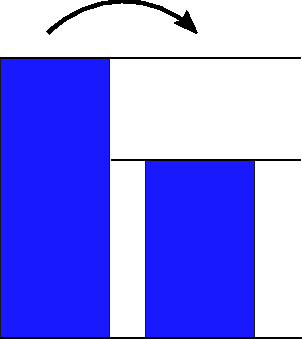
\includegraphics[scale=0.4]{img/pruning.pdf}};
\node (n1) at ( 0.0, 0.85) {$u$};
\node (n2) at ( 0.05, 0.2) {$u'$};
\node (n3) at ( 0.0,-1.0) {$l$};
\node (n4) at (-1.0, 1.5) {pruning by $c_i$};
\node (n5) at (0.8, -0.2) {\large \ldots};
\node (n6) at (6.0, 0.0) {\begin{minipage}{0.7\textwidth}
{\small
\begin{mathpar}
\inferrule{
    \vdots\\
    \inferrule{
        \inferrule{ {} }{ x ∈ [u',u] ∧ c_i \entails ⊥ }{(\thLem)}
    }{
        x ∈ [u',u] ∧ c_i ∧ \bigwedge_{k≠i} c_k \entails ⊥ 
    }{(\weaken)} \\
}{
    x ∈ [l,u] ∧ \bigwedge_k c_k \entails ⊥
}{(\splt)}
\end{mathpar}
}
\end{minipage}
};
\end{tikzpicture}
\caption{
    Pruning operation and the corresponding proof.
    The pruning shrinks the domain of $x$ from $[l,u]$ to $[l,u']$.
    The corresponding proof starts with a \splt around $u'$.
    The interval $[u',u]$ is proved empty using a \thLem and \weaken step.
    The remaining $[l,u']$ interval is shown empty by further operations.
}
\label{fig:prune}
\end{figure}

\section{Interpolants in Nonlinear Theories}
\label{sec:itp}

Intuitively, a proof of unsatisfiability is a partition of the solution space where each sub-domain is associated with a conjunct $c$ from $A ∧ B$.
$c$ is a witness that shows the absence of solution in a given domain.
The interpolation rules traverse the rules and selects which parts belong to the interpolant $I$. We now describe the algorithm for obtaining such interpolants for formulas $A$ and $B$ from the proof of unsatisfiability for $A\wedge B$. 

% need a labelling function
% ThLem: A → false 
%        B → true
% Split: A → I₁ ∨ I₂
%       AB → ite(x_i ≤ p, I₁, I₂) 
%        B → I₁ ∧ I₂
% Weakening: identify

\subsection{Core Algorithms}

\begin{figure}
\centering
\begin{mathpar}
\inferrule{ {} }{
  \vec x ∈ \vec D ∧ c \entails ⊥ \quad [l(c) ≠ \textsc{a}]
}{(\thLemI)}\\

\inferrule{
  C = c ∧ \bigwedge_k C_k \\
  \vec x ∈ \vec D ∧ c \entails ⊥ \quad [I]
}{
  \vec x ∈ \vec D ∧ C \entails ⊥ \quad [I]
}{(\weakenI)}\\


\inferrule{
  x_i ∈ [l_i, p] ∧ \bigwedge_{j ≠ i} x_j ∈ D_j ∧ C \entails ⊥ \quad [I₁] \\\\
  x_i ∈ [p, u_i] ∧ \bigwedge_{j ≠ i} x_j ∈ D_j ∧ C \entails ⊥ \quad [I₂] 
}{
  x_i∈ [l_i, u_i]\wedge \bigwedge_{j\neq i} x_j ∈ D_
  j ∧ C \entails ⊥ \quad
  \left[{\large \substack{ I₁ ∨ I₂     \qquad \quad ~~  \text{if} ~ l(x_i) = \textsc{a} \\
                    ite(x_i < p, I₁, I₂) ~~ \text{if} ~ l(x_i) = \textsc{ab}\\
                    I₁ ∧ I₂     \qquad \quad ~~  \text{if} ~ l(x_i) = \textsc{b}} }\right ]
}{(\spltI)}

\end{mathpar}
where $ite(x,y,z)$ is a shorthand for $(x ∧ y)∨(¬x ∧ z)$
\caption{Interpolant producing proof rules}
\label{fig:rulesI}
\end{figure}

Our method for constructing disjunctive linear interpolants takes two inputs: a proof tree and a labeling function. The labeling function maps formula and variables to either \textsc{a}, \textsc{b}, or \textsc{ab}.
For each proof rule introduced in Figure~\ref{fig:rules}, we associate some partial interpolants, written in square bracket on the right of the conclusion of the rule. 
Figure~\ref{fig:rulesI} shows these modified versions of the rules.
\begin{itemize}
\item At the leaf level (rule \thLemI), the tile is in $I$ if $c$ is not part of $A$, i.e., the contradiction originates from $B$.
If $c$ is in both $A$ and $B$ then it can be considered as either part of $A$ or $B$.
Both cases lead to a correct interpolant.

\item The \weakenI rule does not influence the interpolant, it is only required to pick $c$ from $A ∧ B$.

\item The \spltI is the most interesting rule.
Splitting the domain essentially defines the bounds of the subsequent domains.
Let $x$ be the variable whose domain is split at value $p$ and $I₁$, $I₂$ be the two interpolants for the case when $x < p$ and $x ≥ p$.
If $x$ occurs in $A$ but not $B$, then $x$ cannot occur in $I$.
Since $x$ is in $A$ then we know that $A$ implies $x < p ⇒ I₁$ and $x ≥ p ⇒ I₂$.
Eliminating $x$ gives $I = I₁ ∨ I₂$.
A similar reasoning applies when $x$ occurs in $B$ but not $A$ and gives $I = I₁ ∧ I₂$.
When $x$ occurs in both $A$ and $B$ then $x$ is kept in $I$ and acts as a selector for the values of $x$ smaller than $p$ $I₁$ is selected, otherwise $I₂$ applies.
\end{itemize}
The correctness of our method is shown by the following theorem:
\begin{theorem}
The rules \spltI, \thLemI, \weakenI generate a Craig interpolant $I$ from the proof of unsatisfiability of $A$ and $B$.
\label{thm:sound}
\end{theorem}
\begin{proof}
%\emph{(Sketch)}
We prove correctness of the rules by induction.
To express the inductive invariant, we split the domain $\vec D$ into the domains $\vec D_A$ and $\vec D_B$ which contains only the intervals of the variables occurring in $A$, $B$ respectively.

At any given point in the proof, the partial interpolant $I$ is an interpolant for the formula $A$ over $\vec D_A$ and $B$ over $\vec D_B$.
At the root of the proof tree we get an interpolant for the whole domain $\vec D = \vec D_A ∧ \vec D_B$.

At the leaves of the proof, or the \thLemI rule, one of the constraints has no solution over the domain.
Let's assume that this constraint comes from $A$.
Then the partial interpolant $I$ is $⊥$.
We have that $A ∧ \vec D_A ⇒ I$ by the semantics of the \thLem rule ($⊥⇒⊥$).
Trivially, $B ∧ \vec D_B ∧ I ⇒ ⊥$ and $fv(I) = ∅ ⊆ fv(A) ∩ fv(B)$.
When the contradiction comes from $B$, a similar reasoning applies with $I=⊤$.

The \weakenI only serves to select the constraint which causes the contradiction and does not change the invariant.

The \spltI rule is the most complex case.
We have to consider whether the variable $x$ which is split come from $A$, $B$, or is shared.
For instance, if $x∈ fv(A)$ then the induction step has $\vec D_{A1} = \vec D_A ∧ x < p$ and $\vec D_{A2} = \vec D_A ∧ x ≥ p$ and $\vec D_B$ is unchanged.
If $x ∈ fv(B)$ then $\vec D_B$ is affected and $\vec D_A$ is unchanged.
If $x$ is shared then both $\vec D_A$ and $\vec D_B$ are affected.

Let consider that $x ∈ fv(A)$ and $x ∉ fv(B)$.
We omit the case where $x$ is in $B$ but not $A$ as it is similar.
The induction hypothesis is\\
\parbox{0.35\linewidth}{
\begin{eqnarray*}
& A ∧ (\vec D_A ∧ x < p) ⇒ I₁ \\
& A ∧ (\vec D_A ∧ x ≥ p) ⇒ I₂ \\
& B ∧ \vec D_B ∧ I₁ ⇒ ⊥ \\
& B ∧ \vec D_B ∧ I₂ ⇒ ⊥
\end{eqnarray*}
}
which simplifies to
\parbox{0.35\linewidth}{
\begin{eqnarray*}
& A ∧ \vec D_A ⇒ I₁ ∨ I₂ \\
& B ∧ \vec D_B ∧ (I₁ ∨ I₂) ⇒ ⊥
\end{eqnarray*}
}.

Finally, we need to consider $x ∈ fv(A)$ and $x ∈ fv(B)$.
The induction hypothesis is\\
\parbox{0.38\linewidth}{
\begin{eqnarray*}
& A ∧ (\vec D_A ∧ x < p) ⇒ I₁ \\
& A ∧ (\vec D_A ∧ x ≥ p) ⇒ I₂ \\
& B ∧ (\vec D_B ∧ x < p) ∧ I₁ ⇒ ⊥ \\
& B ∧ (\vec D_B ∧ x ≥ p) ∧ I₂ ⇒ ⊥
\end{eqnarray*}
}
which simplifies to
\parbox{0.42\linewidth}{
\begin{eqnarray*}
& A ∧ \vec D_A ⇒ ite(x < p, I₁, I₂)\\
& B ∧ \vec D_B ∧ ite(x < p, I₁, I₂) ⇒ ⊥
\end{eqnarray*}
}.
\qed
\end{proof}

\begin{example}
If we look at proof for the example in Figure~\ref{fig:example}, we get the proof annotated with the partial interpolants shown in Figure~\ref{fig:proof}.
The final interpolants $I₅$ is $0≤y ∧ (0.26≤y ∨ (y≤0.26 ∧ -0.51 ≤ x ≤ 0.51))$.

\begin{figure}
\centering
\begin{tikzpicture}
\node (box){%
  \begin{minipage}{\textwidth}
{\small
\begin{mathpar}
\inferrule{
    \inferrule{ {} }{
        x ∈ [-0.51,0.51] ∧ y ∈ [0,0.26] ∧ B \entails ⊥ \quad [ ⊤ ]
    }{(\thLemI)}
}{
    x ∈ [-0.51,0.51] ∧ y ∈ [0,0.26] ∧ A ∧ B \entails ⊥ \quad [ I₁: ⊤ ] \\\\ \vdots
}{(\weakenI)}

\inferrule{
    \inferrule{
        \inferrule{ {} }{
            x ∈ [0.51,1] ∧ y ∈ [0,0.26] ∧ A \entails ⊥ \quad [ ⊥ ]
        }{(\thLemI)}
    }{
        x ∈ [0.51,1] ∧ y ∈ [0,0.26] ∧ A ∧ B \entails ⊥ \quad [ ⊥ ]
    }{(\weakenI)} \\
    \vdots ~~ [ I₁ ]
}{
  x ∈ [-0.51,1] ∧ y ∈ [0,0.26] ∧ a ∧ b \entails \bot \quad [ I₂: x≤0.51 ] \\\\ \vdots
}{(\spltI)}

\inferrule{
    \vdots ~~ [ I₂ ] \\
    \inferrule{
        \inferrule{ {} }{
            x ∈ [-1,-0.51] ∧ y ∈ [0,0.26] ∧ A \entails ⊥ \quad [ ⊥ ]
        }{(\thLemI)}
    }{
        x ∈ [-1,-0.51] ∧ y ∈ [0,0.26] ∧ A ∧ B \entails ⊥ \quad [ ⊥ ]
    }{(\weakenI)}
}{
  x ∈ [-1,1] ∧ y ∈ [0,0.26] ∧ a ∧ b \entails \bot \quad [ I₃: -0.51≤x≤0.51 ] \\\\ \vdots
}
        
\inferrule{
    \vdots ~~ [ I₃ ] \\
    \inferrule{
        \inferrule{
            {}
        }{
            x ∈ [-1,1] ∧ y ∈ [0.26,1] ∧ B \entails \bot \quad [ \top ]
        }{(\thLemI)}
    }{
        x ∈ [-1,1] ∧ y ∈ [0.26,1] ∧ A ∧ B \entails \bot \quad [ \top ]
    }{(\weakenI)}
}{
    x ∈ [-1,1] ∧ y ∈ [0,1] ∧ A ∧ B \entails \bot \quad [ I₄: ~ 0.26 \leq y \lor (y \leq 0.26 ∧ I₃) ] \\\\ \vdots
}{(\spltI)}

\inferrule{
    \inferrule{
        \inferrule{
            {}
        }{
            x ∈ [-1,1] ∧ y ∈ [-1,0] ∧ A \entails \bot \quad [ \bot ]
        }{(\thLemI)}
    }{
        x ∈ [-1,1] ∧ y ∈ [-1,0] ∧ A ∧ B \entails \bot \quad [ \bot ]
    }{(\weakenI)} \\
    \vdots ~~ [ I₄ ]
}{
    x ∈ [-1,1] ∧ y ∈ [-1,1] ∧ A ∧ B \entails \bot \quad [ I₅: ~ 0 \leq y ∧ I₄ ]
}{(\spltI)}
\end{mathpar}
}
  \end{minipage}
};
\draw [loosely dotted,thick] plot [smooth,tension=1] coordinates { (-0.95,4.4) (-0.0,4) (3.2,4.0) (4.1,3.4) } ;
\draw [loosely dotted,thick] plot [smooth,tension=1] coordinates { (-0.55,1.5) (-1.5,1.2) (-4.2,1.2) (-5.63,0.6) } ;
\draw [loosely dotted,thick] plot [smooth,tension=1] coordinates { (-0.0,-1.35) (-1.2,-1.8) (-4.5,-1.8) (-5.85,-2.3) } ;
\draw [loosely dotted,thick] plot [smooth,tension=1] coordinates { (-0.55,-4.2) (0.3,-4.6) (3.0,-4.6) (3.96,-5.15) } ;
\end{tikzpicture}
\caption{Proof of unsatisfiability where $A$ is $y≥x²$, $B$ is $y ≤ -\cos(x) + 0.8$ along with the corresponding interpolant}
\label{fig:proof}
\end{figure}
\end{example}

\paragraph{Boolean structure.}
The method we presented explain how to compute an interpolant for the conjunctive fragment of quantifier-free nonlinear theories over the reals.
However, in many cases formula also contains disjunctions.
To handle disjunctions, our method can be combined with the method presented by Yorsh and Musuvathi~\cite{DBLP:conf/cade/YorshM05} for building an interpolant from a resolution proof where some of the proof's leaves carry theory interpolants.

\paragraph{Handling ODE constraints.} A special focus of delta-complete decision procedures is on constraints that are defined by ordinary differential equations, which is important for hybrid system verification. In the logic formulas, the ODEs are treated simple as a class of constraints, over variables that represent both state space and time. Here we elaborate on the proofs and interpolants for the ODE constraints.  

 Let $t_0, T\in \mathbb{R}$ and $g:\mathbb{R}^n\rightarrow \mathbb{R}$ be a Lipschitz-continuous Type 2 computable function. Let $t_0, T\in \mathbb{R}$ satisfy $t_0\leq T$ and $\vec x_0\in \mathbb{R}^n$. Consider the initial value problem
\[\frac{\mathrm{d}\vec x}{\mathrm{d}t} = \vec g(\vec x(t))\mbox{ and } \ \vec x(t_0) = \vec x_0, \mbox{ where }t\in [t_0, T].\]
It has a solution function $\vec x: [t_0, T]\rightarrow \mathbb{R}^n$, which is itself a Type 2 computable function~\cite{CAbook}. Thus, in the first-order language $\lrf$ we can write formulas like
\[\Big(||\vec x_0||=0\Big) \wedge\Big( \vec x_t = \vec x_0+\int_0^t \vec g(\vec x(s))\mathrm{d}s\Big) \wedge\Big(||\vec x_t|| > 1\Big)\]
which is satisfiable when the system defined by the vector field $\vec g$ can have a trajectory from some point $||\vec x(0)||=0$ to $||\vec x(t)||=1$ after time $t$. Note that we use first-order variable vectors $\vec x_0$ and $\vec x_t$ to represent the value of the solution function $\vec x$ at time $0$ and $t$. Also, the combination of equality and integration in the second conjunct simply denotes a single constraint over the variables $(\vec x_0, \vec x_t, t)$. 

In the $\delta$-decision framework, we perform interval-based integration for ODE constraints that satisfies the following. Suppose the time domain for the ODE constraint in question is in $[t_0,T]$. Let $t_0\leq t_1\leq \cdots t_m\leq T$ be a sequence of time points. An interval-based integration algorithms compute boxes $D_{t_1},...,D_{t_m}$ such that 
$$\forall i\in \{1,...,m\},\; \{\vec x(t): t_i\leq t\leq t_{i+1}, \vec x_0\in D_{\vec x_0}\}\subseteq D_{t_0}.$$
Namely, it computes a sequence of boxes such that all possible trajectories are containted in them over time. Thus, the ODE constraints can be handled in the same way as non-ODE constraints, whose solution set is covered by a set of small boxes. Consequently, the proof rules from Figure~\ref{} apply directly to ODE constraints. 







\subsection{Extensions}

%When using interpolation as an heuristic to accelerate fixed point computation for verification,
For any two formulas $A$,$B$ which conjunction is unsatisfiable, the interpolant $I$ is not unique.
In practice, it is difficult to know a priori what is a good interpolant.
Therefore, it is desirable to have the possibility of generating and testing multiple interpolants.
We now explain how to get multiple interpolant of different logical strength.

\paragraph{Parameterizing interpolation strength.}

The interpolation method that we propose uses a δ-decision procedure to build a Craig interpolant.
$I$ being an interpolant means that $A ∧ ¬I$ and $B ∧ I$ are both unsatisfiable.
However, these formulas might still be δ-satisfiable.

To obtain an interpolant such that both $A ∧ ¬I$ and $B ∧ I$ are δ-unsatisfiable, we can weaken both $A$ and $B$ by a factor δ.
However, $A$ and $B$ must be at least $3δ$-unsatisfiable to guarantee that the solver finds a proof of unsatisfiability.
Furthermore, we can also introduce perturbations only on one side in other to make the interpolant stronger of weaker.
To introduce a perturbation δ, we apply the following rewriting to every inequalities in $A$ and/or $B$:
\begin{eqnarray*}
L = R & ~~ \mapsto ~~ & L ≥ R - δ ∧ L ≤ R + δ \\
L ≥ R & ~~ \mapsto ~~ & L ≥ R - δ \\
L > R & ~~ \mapsto ~~ & L > R - δ \\
\end{eqnarray*}

\paragraph{Changing the labelling.}
%\todo{this paragraph could use a better explanation}
Due to the similarity of our method to the interpolation of propositional formulas we can adapt the labelled interpolation system from D'Silva et.al.~\cite{DBLP:conf/vmcai/DSilvaKPW10} to our framework.

In the labelled interpolation system, it is possible to modify the \textsc{a,b,ab} labelling as long as it preserves \emph{locality}, see \cite{DBLP:conf/vmcai/DSilvaKPW10} for the details.
An additional restriction in our case is that we cannot use a projection of constraints at the proof's leaves.
The projection is not computable in nonlinear theories.
Therefore, the labelling must enforce that the leaves maps to the interpolants ⊤ or ⊥.

\section{Examples and Experiments}
\label{sec:eval}

We have implemented the interpolation algorithm in a modified version of the \dReal which is available at \url{https://github.com/dzufferey/dreal3/}.
The interpolation hooks at the places where the proof is produced.
Since the proofs produced by \dReal can be very large,i.e., gigabytes, the interpolants are built and simplified on-the-fly.
The full proof is not kept.


\section{Conclusion}
\label{sec:concl}

We present an method for computing Craig interpolants for first-order formulas over real numbers with a wide range of nonlinear functions.
Our method transform proof traces from δ decision procedures into interpolants consisting of disjunctive linear constraints.
The algorithms are guaranteed to find the interpolants between two formulas $A$ and $B$ whenever $A ∧ B$ is not δ-satisfiable.
Furthermore, we show how the framework apply to systems of ordinary differential equations.
We implemented our interpolation algorithm in the \dReal SMT-solver and apply the method to domains such robotic design, and hybrid system verification.  


\bibliographystyle{abbrv}
\bibliography{biblio,refs}

\appendix
%\section{Proofs}

TODO better formating ...

Correctness of the interpolation rules:

Proof by induction.

\paragraph{Base case: \textsc{ThLemI} rule}
if $l(f)=A$ and $I=⊥$ then
\begin{itemize}
\item $A ⇒ I$: if $l(f)=A$ the theroy lemma means that $A⇔⊥$, thus, $⊥⇒⊥$
\item $B ∧ I ⇒ ⊥$: trivially $⊥⇒⊥$
\item $fv(I) ⊆ fv(A) ∩ fv(B)$: trivial
\end{itemize}

else we have $l(f)=B$ and $I=\top$, so
\begin{itemize}
\item $A ⇒ I$: trivially $\top ⇒ \top$
\item $B ∧ I ⇒ ⊥$:  if $l(f)=B$ the theroy lemma means that $A⇔⊥$, thus, $⊥⇒⊥$
\item $fv(I) ⊆ fv(A) ∩ fv(B)$: trivial
\end{itemize}

\paragraph{Induction step 1: \textsc{WeakeningI} rule}
\begin{itemize}
\item $A ⇒ I$: by induction hypothesis
\item $B ∧ I ⇒ ⊥$: by induction hypothesis
\item $fv(I) ⊆ fv(A) ∩ fv(B)$: by induction hypothesis
\end{itemize}

\paragraph{Induction step 2: \textsc{SplitI} rule}
The trick is how to apply the induction hypothesis.
We have to consider 3 cases:
\begin{enumerate}
\item $x ∈ fv(A) ∧ x \notin fv(B)$ and $I = I₁ ∨ I₂$
\item $x ∈ fv(A) ∧ x ∈ fv(B)$ and $I = ite(x < p, I₁, I₂)$
\item $x \notin fv(A) ∧ x ∈ fv(B)$ and $I = I₁ ∧ I₂$
\end{enumerate}

Let's divide the domain $D$ into $D_A$ and $D_B$ where each contains the range of the corresponding variables.
Variables that are in both side have their domain in both $D_A$ and $D_B$. 
if $x\in fv(A)$ then the induction step has $D_{A1} = D_A ∧ x < p$ and $D_{A2} = D_A ∧ x ≥ p$ and $D_B$ is unchanged.

In the first case, the induction hypothesis is
\begin{eqnarray*}
& A ∧ x_i < p ⇒ I₁ \\
& A ∧ x_i ≥ p ⇒ I₂ \\
& B ∧ I₁ ⇒ ⊥ \\
& B ∧ I₂ ⇒ ⊥
\end{eqnarray*}
which simplifies to:
\begin{eqnarray*}
& A ⇒ I₁ ∨ I₂ \\
& B ∧ (I₁ ∨ I₂) ⇒ ⊥
\end{eqnarray*}

In the second case, the induction hypothesis is
\begin{eqnarray*}
& A ∧ x_i < p ⇒ I₁ \\
& A ∧ x_i ≥ p ⇒ I₂ \\
& B ∧ x_i < p ∧ I₁ ⇒ ⊥ \\
& B ∧ x_i ≥ p ∧ I₂ ⇒ ⊥
\end{eqnarray*}

The first two equations gives
\[
    ¬ A ∨ (¬(x < p) ∨ I₁) ∧ (¬(x ≥ p) ∨ I₂)
\]
which is the same as $¬ A ∨ ite(x < p, I₁, I₂)$
and, therefore, $A ⇒ ite(x < p, I₁, I₂)$.

The last two equations gives
\[
    ¬ B ∨ ((¬(x < p) ∨ ¬ I₁) ∧ (¬(x ≥ p) ∨ ¬ I₂))
\]
using distributivity law we get
\[
    ¬ B ∨ (x ≥ p ∧ ¬ I₂) ∨ (x < p ∧ ¬ I₁) ∨ (¬ I₁ ∧ ¬ I₂)
\]
because $(¬ I₁ ∧ ¬ I₂) ⇒  (x ≥ p ∧ ¬ I₂) ∨ (x < p ∧ ¬ I₁)$
this simplifies to
\[
 ¬ B ∨ (x ≥ p ∧ ¬ I₂) ∨ (x < p ∧ ¬ I₁)
\]
which is the same as: $¬ B ∨ ¬ ite(x < p, I₁, I₂)$
and, therefore, $B ∧ ite(x < p, I₁, I₂) ⇒ ⊥$.

In the third case: the induction hypothesis is
\begin{eqnarray*}
& A ⇒ I₁ \\
& A ⇒ I₂ \\
& B ∧ x_i < p ∧ I₁ ⇒ ⊥ \\
& B ∧ x_i ≥ p ∧ I₂ ⇒ ⊥
\end{eqnarray*}
which simplifies to:
\begin{eqnarray*}
& A ⇒ I₁ ∧ I₂ \\
& B ∧ (I₁ ∧ I₂) ⇒ ⊥
\end{eqnarray*}




\end{document}

